\section{Reinforcement Learning for Reasoning Skill Refinement}
\begin{frame}[allowframebreaks]{}
    \LARGE Reinforcement Learning for Reasoning Skill Refinement
\end{frame}

\begin{frame}{Reinforcement Learning with Verifiable Rewards}
    \begin{itemize}\itemsep0.3em
        \item Reasoning tasks have a property alignment tasks lack: correctness can be \emph{checked}. A final answer matches the key, unit tests pass, a proof term type-checks.
        \item \textbf{RL with verifiable rewards (RLVR)} puts that checker where the learned reward model used to be: the reward is a program, not a network.
        \item One step: sample a group of complete traces for a prompt, run the checker on each, then shift probability mass toward the traces that passed.
        \item Upside: no reward model to train or hold in memory, nothing to hack short of the checker itself, and a reward that stays correct however far the policy drifts from the SFT model.
        \item Downside: one bit per trace, and nothing until it finishes, so credit for a fifty-step derivation rests on the last line. The method also reaches only as far as checkers do, leaving open-ended writing and judgement calls to preference-based training.
    \end{itemize}
\end{frame}

\begin{frame}[allowframebreaks]{RLVR with Very Few Training Examples}
        \begin{figure}[h]
            \centering
            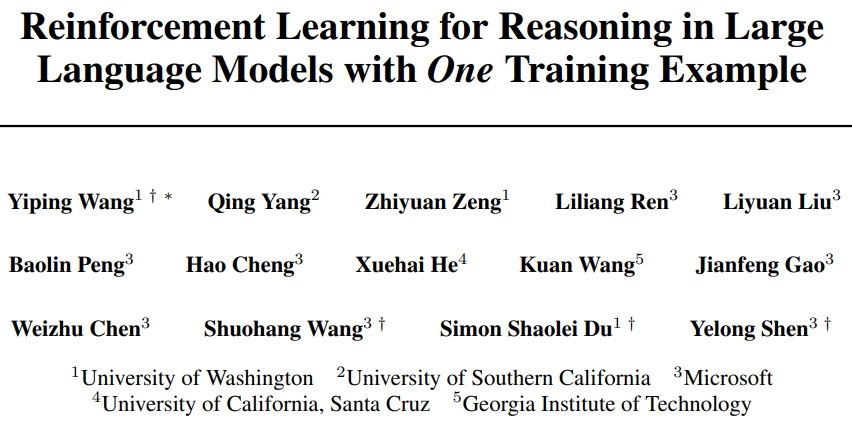
\includegraphics[width=\textwidth,height=0.84\textheight,keepaspectratio]{images/lrm+moe/paper-rl-for-reasoning-llm.png}
            \caption*{Source: \href{https://arxiv.org/abs/2504.20571}{Wang et al. (2025)}}
        \end{figure}
    \framebreak
        \begin{figure}[h]
            \centering
            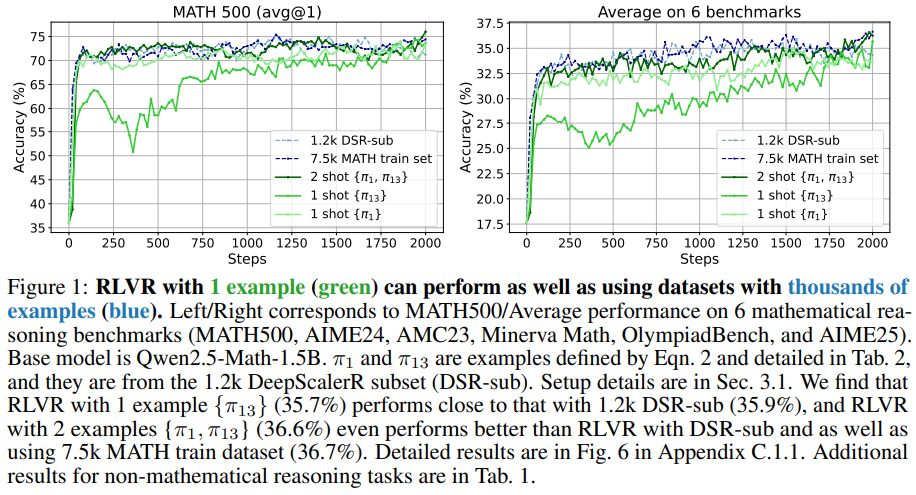
\includegraphics[width=\textwidth,height=0.84\textheight,keepaspectratio]{images/lrm+moe/rlvr-dataset-result.png}
            \caption*{Source: \href{https://arxiv.org/abs/2504.20571}{Wang et al. (2025)}, Fig.~1.}
        \end{figure}
    \framebreak
        \begin{figure}[h]
            \centering
            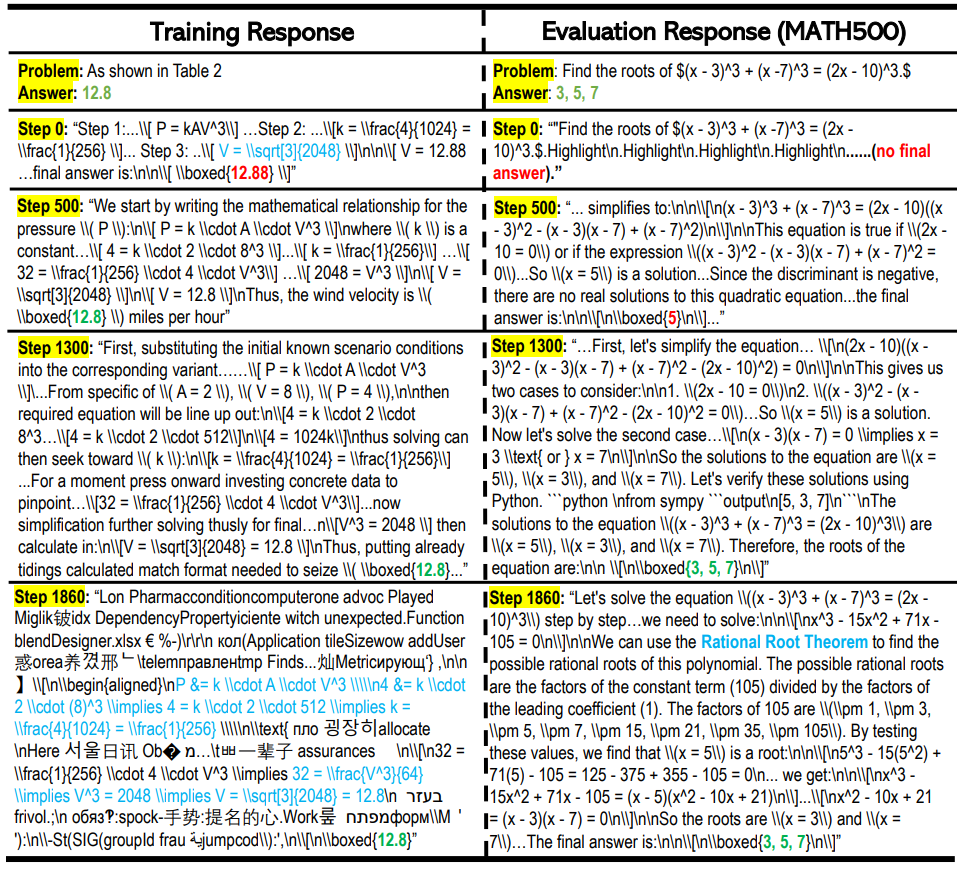
\includegraphics[width=\textwidth,height=0.78\textheight,keepaspectratio]{images/lrm+moe/rlvr-result.png}
            \caption*{Model's response to training example $\pi_1$ and a selected MATH500 problem. Green/Red are used for marking Correct/Wrong answers. Source: \href{https://arxiv.org/abs/2504.20571}{Wang et al. (2025)}, Fig.~3.}
        \end{figure}
    \framebreak
        \begin{figure}[h]
            \centering
            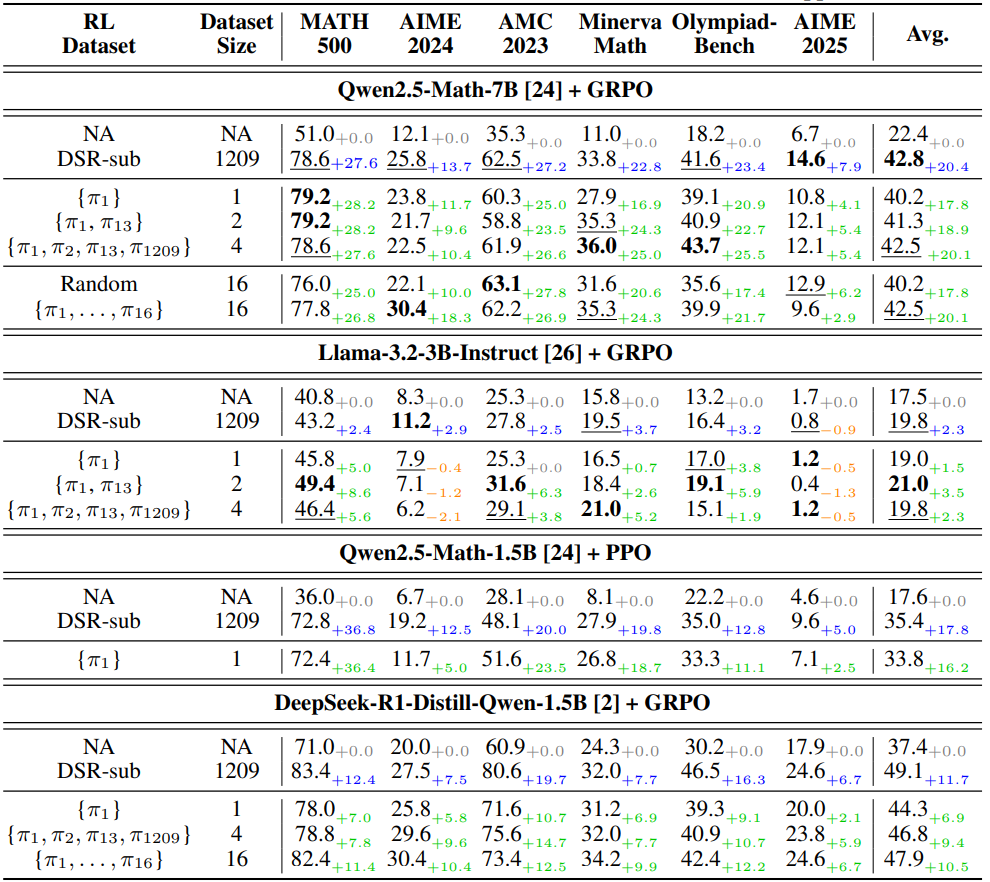
\includegraphics[width=\textwidth,height=0.78\textheight,keepaspectratio]{images/lrm+moe/rlvr-viability.png}
            \caption*{1(few)-shot RLVR is viable for different models and RL algorithms. Source: \href{https://arxiv.org/abs/2504.20571}{Wang et al. (2025)}, Tab.~4.}
        \end{figure}
\end{frame}

\begin{frame}{Outcome Rewards vs Process Rewards}
  \begin{itemize}\itemsep0.4em
    \item[\textcolor{red}{$\blacktriangleright$}] \textbf{Outcome reward models (ORMs)} score only the final result: is the answer correct, do the tests pass?
    \item[\textcolor{red}{$\blacktriangleright$}] \textbf{Process reward models (PRMs)} score every intermediate step of the reasoning trace. Training them requires step-level labels (Lightman et al., 2023, ``Let's Verify Step by Step'', with the PRM800K dataset of human step annotations).
    \item[\textcolor{red}{$\blacktriangleright$}] PRMs give denser feedback and catch correct answers reached by invalid reasoning; ORMs are cheaper, and in verifiable domains need no trained model at all, since a rule or checker suffices.
    \item[\textcolor{red}{$\blacktriangleright$}] PRMs carry their own risks: step labels are expensive, step correctness is hard to define outside mathematics, and step-level supervision can penalize unconventional but valid reasoning paths.
    \item[\textcolor{red}{$\blacktriangleright$}] DeepSeek-R1 chose rule-based outcome rewards after finding that process rewards constrained exploration and invited reward hacking.
  \end{itemize}
\end{frame}
